\documentclass{apa6e}
\usepackage{apacite} % This is not done automatically!
\usepackage{graphicx}
\bibliographystyle{apacite}
\title{Computational emotional thinking via virtual hormones}
\shorttitle{Computational Emotional thinking}
\author{Max ~Talanov and Alexander ~Toschev\\Higher Institute of Information Technologies and Information Systems of \\Kazan Federal University}
\authornote{Correspondence concerning this article should be addressed to Max Talanov,
e-mail: max.talanov@gmail.com or Alexander Toschev, e-mail: sanchis@gmail.com}
\abstract{Our work is dedicated to construction or synthesis of computational emotional thinking model.
We used 4 basis for our work: AI - six thinking levels model described in book "The emotion machine" \cite{emotionmachine}. Evolutionary psychology model of emotions that is called "Wheel of emotions"\cite{natureofemotions}, we used as subjective perception model. Neuroscience(neurotransmission) theory of emotions by L\"{o}vheim "Cube of emotions"\cite{cubeofemotions} was used as objective brain emotional response model. Based on neurotransmitters impact we propose to model emotional computing systems. Overall presented work is synthesis of several emotional/affective theories to produce model of emotions and affective mechanisms that fit model of six thinking levels architecture.\\
Keywords: Emotion, Affect, Computing, AI, Neuromodalation, Neurotransmission, Model of Emotions, Cognitive and Affective Modelling, Thinking }
\begin{document}
\begin{center}
Invited Paper.\\
\end{center} 
\maketitle
Today emotions are in focus of a lot of researchers from neuro-scientists \cite{emotionsbraintorobot, parsingreward, neuromodulatory, cubeofemotions}, to computer science specialists \cite{emotionandsociable, senticcomputing, hourglass, affectivemodelofinterplay, affectivecomputing, affectivecomputingchallanges}.
There were only some computational emotions models created \cite{computationalmodelsemotion, computationalmodelsemotionscognition, evaluatingcomutationalmodel, threelevel} and we failed to find a computational emotion thinking model already created. Marvin Minsky in his book "The emotion machine" \cite{emotionmachine} described a human thinking model, and proposed a promising base for emotional thinking implementation in computing systems. He demonstrated that emotions are inseparable parts of thinking "Emotional thinking: A flash of impatience or anger can cut through what seems like a hopelessly tangled knot. Each such ‘emotional way to think' is a different way to deal with things, and some can increase your persistence or courage, while others can help you simplify things.
In any case, after each such change, you may still want to pursue some similar goals, but now you’ll see them from new points of view — because each switch to a new Way to Think may initiate a large-scale cascade. Then, depending on how long those changes persist, you (or your friends) might recognize this as a change in your emotional state". Robert Plutchik in his article "The nature of emotions" \cite{natureofemotions} states that emotions evolved through years and became important part of cognitions, behaviour and mind "What we call cognition — the activity of knowing, learning and thinking, of which emotion is a part — evolved over millions of years. Charles Darwin recognized that the process of evolution by natural selection applied not only to anatomic structures but also to an animal's "mind" and expressive behavior — a conclusion that led him to write a book on emotional expression. Those who have followed Darwin in studying the evolutionary origins of emotion have sought to understand how emotions increase evolutionary fitness for the individual". Hence because - there is no example of unemotional intelligence and emotions are an inseparable part of thinking we face the problem of emotional thinking model implementation as soon as we attempt to construct a system that is more or less comparable to human intelligence. This is interdisciplinary work that we have run to create theoretical basis for computational emotional thinking to be used further for modelling and implementing as code and possible embodiment in social robot. There could be selected several domains for future use: computer - human social collaboration, human emotional behaviour assessment, computer games and simulations, automation of primitive service tasks, nursing.

\section{Emotional thinking model}

\subsection{Minsky's Thinking model}

First basis is  AI. Marvin Minsky in his book "The emotion machine" \cite{emotionmachine} described human thinking model. Main structural idea that we adopted is "Model of six" contains following levels: 
\begin{enumerate}
\item  Instinctive reactions
\item  Learned reactions
\item  Deliberative
\item  Reflective thinking
\item  Self-reflective thinking
\item  Self-conscious reflections
\end{enumerate}

This way all emotional processes should be expressed in terms of thinking model(levels). This could be understood as the base of computational emotional thinking approach.

\subsection{Evolutionary psychology}

We use Plutchik approach \cite{natureofemotions} as main psychological model. Plutchik indicated 8 basic emotions grouped in 4 pairs:

\begin{enumerate}
\item  Joy - sorrow
\item  Anger - fear
\item  Acceptance - disgust
\item  Surprise - expectancy
\end{enumerate}

Emotions are organised in three dimensional circumplex model, where third dimension is emotional strength. Basic emotions could be mixed based on color theory, in complex emotions that are called "primary dyads": love, submission, awe, disapproval, remorse, contempt, aggressiveness, optimism. More complex emotions based on three basic emotions could be combined in similar way, see Cambria \cite{senticcomputing}. Cambria \cite{hourglass} used Gauss function to describe passage from one sentic level to another. We interpreted it as: Gaussian function regulates influence of subjective human perception of inbound stimulus over objective brain response. Semir Zeki \cite{neuralcorrelatesofhate} describes emotion(hate) correlation to neural activities as Gaussian.

\subsection{Neuromodulation and neurotransmission theory}

Objective brain work is described as neuromodulation process in \cite{neuromodulatory} and \cite{emotionsbraintorobot}.
Close to their work is model based on monoamine neurotransmitters called "Cube of emotions" of Hugo L\"{o}vheim \cite{cubeofemotions} with three main neurotransmitters: nor-adrenaline, dopamine, serotonin. L\"{o}vheim assumes that all emotional states could be placed in the three dimensional cube with neurotransmitters as axes and eight basic emotions ordered in an orthogonal coordinate system. Emotional states are inherited from affect theory of Tomkins \cite{tomkins1, tomkins2, tomkins3}:enjoyment/joy, interest/excitement, surprise, anger/rage, disgust, distress/anguish, fear/terror, shame/humiliation. This group of affects matches  Plutchik's basic emotions model except for same-humiliation that could be interpreted as remorse.\\
According to \cite{emotionsbraintorobot} neuronal systems involved in emotional processing are: spinal cord, hypothalamus, amygdala, frontal cortex and cingulate cortex. We correspond spinal cord, hypothalamus and amygdala with instinctive layer of Minsky's thinking model. This mapping is done in the assumption that reflexes, drives and instincts could be placed in instinctive reactions layer responsible for most primitive non-conscious actions. Cognitions are placed in 5 higher layers that corresponds to working memory.

\subsection{Emotions in six thinking levels}

We described Plutchik's feedback loops \cite{natureofemotions} in Minsky's six thinking levels (see Figure 1. Emotions in model of six thinking levels).

First \emph{inbound stimulus} is processed via spinal cord, hypothalamus, amygdala and all these neuronal systems take part in neuromodulation. 
\emph{Neuromodulation} actually triggers the emotional state of human and all the rest actions are done under the influence of neuromodulatory systems: nor-adrenaline, dopamine, serotonin. 
\emph{Instinctive behavior} is triggered on an instinctive reactions layer that is not involved in conscious actions. 
Result of behavior is \emph{effect} state that influences the system again as stimulus. This second stimulus is appraised on instinctive reactions layer and triggers neuromodulation again. Neuromodulation in its turn switches emotional state second time. This way stimulus cognition actions started in first emotional state, could continue in second emotional state. 
\emph{Stimulus cognition} is processed in cingulate cortex, frontal cortex (working memory) that corresponds to rest 5 layers of thinking model. Stimulus cognition actions is done in the emotional state under the influence of neuromodulation. Stimulus cognition could involve deliberation, further reflection, sef-reflection self-conscious processing (higher emotions) and  emotional state switch.
\emph{Conscious behavior} is activated as the result of stimulus cognition.

\subsubsection{Stimulus appraisal and stimulus cognition}

There are two main ways of inbound stimulus processing: appraisal is done on the instinctive reactions level, cognition could involve all the rest thinking levels and could consist of complex deliberations and reflections.
Cognitions also include self-conscious reflections over complex emotions like love, awe and aggression. For example \emph{startle} is been apprised on instinctive reactions layer (spinal cord, hypothalamus, amygdala) where non-conscious decision is made and instinctive behaviour is chosen (it could be even reflex). In case of startle this could be run. Only after those instinctive actions are performed human could realise what had happened to him/her (in the state of effect). In contrast to appraisal cognitions that are performed on higher levels could take some significant time and include complex reasoning and reflections. For example fear could be triggered by inbound stimulus and by long time perception during some horror movie or deliberation over some facts regarding the world. In contrast to startle, fear triggers complex conscious behaviour that could in its turn become panic and trigger less intelligent behaviour like shouting and running from side to side. Both instinctive and conscious behaviour produces effect state. Effect is an environmental state that was altered from previous state via behaviour. Running in case of startle places human in safe place that produces effect which influence stimulus event and its appraisal and as consequence emotional/affective state.

\subsubsection{Feeling the state and neuromodulation}

Feeling the emotional state is closely related to neuromodulation the physiological arousal processes in brain. The result of stimulus appraisal is subjective emotional state one of 8 basic Plutchik emotions that are used as dimensions and strength of emotion. This way subjective emotional state is expressed via two coordinates: emotional state nature and strength of emotion. Emotional state nature and emotional strength are in range from 0 to 1. Subjective strength of emotion corresponds to objective brain activities via Gaussian function see \cite{hourglass}. Objective brain activities are expressed via neuromodulation, see \cite{emotionsbraintorobot} that is expressed in terms of neurotransmitters concentration. Neurotransmitters  concentration is expressed in range from 0 to 1 in cube of emotions, see L\"{o}vheim \cite{cubeofemotions}. This way inbound stimulus is been apprised and triggers subjective emotional state switch and then objective brain functions as result of neurotransmitters concentration variation. For example the system is scared. The system switched its state to terror with maximum strength 1. This subjective terror strength is mapped to objective dopamine(neurotransmitter) concentration, in our case this is maximum 1. Under the influence of maximum concentration of dopamine all further actions is performed: decisions over instinctive behavior, stimulus cognitions, selection of conscious behavior. All higher thinking processes control and influence lower actions. For example: if human is scared during watching a film he/she usually does not jump and run away. Some kind of reflection(reflection thinking level) is used: "This is just a movie, nothing terrible is going to happen to me". This is done by switching emotional state on reflection thinking level.

\subsubsection{Neuromodulation to computing system management mapping}

All that was presented above was the description of human thinking process and human emotions in terms of it. Only one reference to AI was done by Marvin Minsky in "The emotion machine" \cite{emotionmachine}. Result of neuromodulation is neurotransmitters secretion. Roughly we could state that noradrenaline influences overall speed of thinking process, dopamine and serotonin - reward processing and learning(see Figure 2 Computing system parameters mapping).

Serotonin takes part in: behavioral state regulation and arousal, motor pattern generation, learning and plasticity, mood and social behavior \cite{anatomic} also in self confidence, inner strength, satisfaction \cite{cubeofemotions}. Dopamine plays a major role in motor activation, reward processing, reinforcement, motivation (wanting) \cite{cubeofemotions, emotionsbraintorobot, roleofemotions}. Noradrenaline impacts attention, vigilance, activity \cite{cubeofemotions}.

Parameters are grouped in two folders: most obvious computing system parameters (generic):
\emph{CPU power}(computing processes distribution or load balancing) is influenced by noradrenaline the higher is noradrenaline more computing processes should be concentrated on current activity.
\emph{Working memory(short term)} distribution is influenced by noradrenaline as neurotransmitter regulating attention.
\emph{Learning} is impacted by serotonin and dopamine: dopamine plays major role in activation of previously remembered patterns and serotonin in pattern generation.
\emph{Storage} management (long term memory) is influenced both by serotonin and dopamine, higher concentrations of both neurotransmitters the better action is remembered(less probability to forget).

Second group contains parameters that influence decision making in probabilistic reasoning system. This reasoning is done mainly in deliberation and learned reaction layers.
Parameters: confidence, satisfaction, risky are used to highlight actions stored(remembered).
\emph{Confidence and satisfaction} of the system is directly influenced by serotonin: the higher serotonin more confident is the system. 
The system is more \emph{motivated} under influence of dopamine.
The system tends to choose \emph{risky} actions under impact of noradrenaline.
Noradrenaline makes system use less \emph{number of options} in width and depth to be processed during reasoning.

For example: system is in fear state. Dopamine impacts system at half strength. This makes system choose actions highlighted with high rewards(safest in case of fear). High noradrenaline in rage state causes system to think as quickly as possible taking in account as less as possible number of options, implementing first action(usually not really safe) selected "fight or flight" reaction.

It is worth to note that duration of each neurotransmitter impact is highly individual and requires further development from a computing system development perspective. Currently we suppose that each neurotransmitter is terminated right after it impacts the system.

\subsubsection{Conformity with Picard criteria}

Rosalind Picard in her article "What does it mean for a computer to "have" emotions?" \cite{whatdoesitmeanforcomputer} suggested following criteria to measure emotional capabilities of a computing system:

\begin{enumerate}
\item  Emotional appearance
\item  Multi-level emotion generation
\item  Emotional experience
\item  Mind-body interactions
\end{enumerate}

Emotional appearance is not discussed in this work. Multi-level emotion cognition and behavior generation was demonstrated in "Emotions in six thinking levels" and "Feeling the state and neuromodulation" sections. Emotional experience is complex that consists of: "cognitive or semantic label; physiological changes; subjective feeling, intuition" we have scratch the surface and suggested psychological changes mechanism according to Plutchik model and subjective emotions perceptions in this work. Mind-body interactions consists of: "conscious and non-conscious events; regulatory and signaling mechanisms; biasing mechanisms, intuition; physiological and biochemical changes; sentic modulation, lying impacts pressure; waveform of love; smiles induce joy..." this partly could be implemented by presented model. Conscious and non-conscious mechanisms of stimulus processing was presented in "Stimulus appraisal and stimulus cognition" section. Psychological and biochemical changes where presented in "Feeling the state and neuromodulation" and "Neuromodulation to computing system management mapping".

\subsubsection{Higher emotions}

Plutchik \cite{natureofemotions} suggested "primary dyads", see "Evolutionary psychology" section above, could be produced as mixture of primary colors of basic emotions. For example: joy(yellow) plus trust(green) produces love(lemon), anger(red) plus disgust(lilac) produces contempt(violet). Higher or complex emotions requires higher levels of thinking and self-awareness to be involved, this way they are mainly triggered on self-conscious and self-reflective thinking levels. Triads could be produced in similar way to dyads: joy + trust + anger = jealousy, see \cite{senticcomputing}.

\section{Conclusion}

Emotions are part of human thinking. In this paper we presented three bases for a computational emotions model. Firstly from AI, Marvin Minsky "The emotion machine" \cite{emotionmachine} thinking model (model of six), evolutionary psychological model: "wheel of emotions" by Plutchik \cite{natureofemotions} is as subjective emotional state mode, objective emotional brain activity is modelled by "cube of emotions" the monoamine neurotransmitters emotions model. We presented parameters of computing system management with mapping to monoamine neurotransmitters. This approach could be used for further implementation as emotional thinking process, framework for general AI applications. We suppose that this model is worth testing in computing system built on a base of six levels. For example, it could be automation of help desk. More than that we could run interesting experiment switching on and off emotions mechanisms, for example neurotransmitters in the system and monitoring efficiency of cognition and training processes. Emotional thinking process implementation could be useful in many different domains: computer games, intellectual assistants, automatic interviewers, estimating human responses, simulations of large social groups, call centre and software support automation, virtual friends and nursing software, applications in emotional robots.

\begin{figure}[h!]
 \centering
 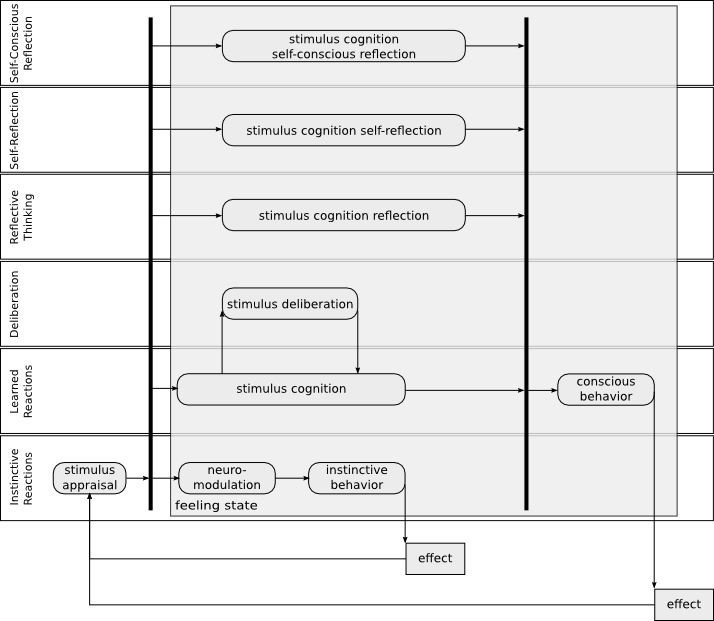
\includegraphics[width=0.7\textwidth]{six_levels_of_emotions}
 \caption{[Emotions in model of six thinking levels].}
\end{figure}

\begin{figure}[h!]
 \centering
 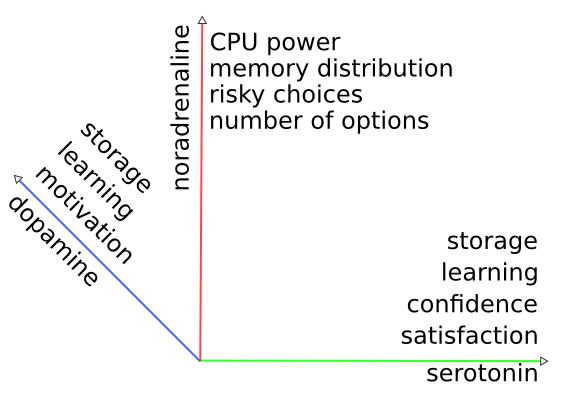
\includegraphics[width=0.3\textwidth]{parameters_mapping180}
 \caption{[Computing system parameters mapping].}
\end{figure}
\bibliography{ref}
\end{document}